\section{Results}
After creating and validating or model, we collected exprimental data for a triple pendulum which had been constructed by Ben Smith for the course.  The parameters of this experimental test setup were measured (Table \ref{expparams}) and input into our simultaion.  The triple pendulum was tracked by an OptiTrack vision tracking system and the data was parsed with a Python script in order to return angles as functions of time for the three links.  This vision tracking was set up by professor Aaron Hoover.  Velocity data for the three links was created through numerical differentiation and a low-pass filter using MATLAB's filter function.

\begin{table}[H]
\centering
 \begin{tabular}{|l|l|l|}
        \hline
        Parameter & Value    & Unit        \\ \hline
        $m_1$     & 0.2944   & kg          \\ 
        $m_2$     & 0.1756   & kg          \\ 
        $m_3$     & 0.0947   & kg          \\ 
        $l_1$     & 0.508    & m           \\ 
        $l_2$     & 0.254    & m           \\ 
        $l_3$     & 0.127    & m           \\ 
        $I_1$     & 9.526e-3 & kg$\cdot$ m^2 \\ 
        $I_2$     & 1.625e-3 & kg$\cdot$ m^2 \\ 
        $I_3$     & 1.848e-4 & kg$\cdot$ m^2 \\ 
        $k_1$     & 5e-3     & N$\cdot$m$\cdot$s/rad           \\ 
        $k_2$     & 0        & N$\cdot$m$\cdot$s/rad           \\ 
        $k_3$     & 8e-4     & N$\cdot$m$\cdot$s/rad           \\
        \hline
    \end{tabular}
    \caption{Parameters of Experimental Triple Pendulum System}
    \label{expparams}
\end{table}

We ran the experiment for a number of varying initial conditions, some which would create chaotic and some which would create periodic motion from the start.  We used one of the periodic cases (Table \ref{initials}) to validate our simulation and tune the damping constants ($k_n$).  The position and velocity of each of the three links was plotted as a function of time and the damping constants were tuned until the positional and velocity plots closely matched the experimental data.  The final values for the damping constants ($k_n$) are given in Table \ref{expparams}.

\begin{table}[H]
\centering
 \begin{tabular}{|l|l|l|}
        \hline
        Condition  & Value  & Unit        \\ \hline
        $\theta_1$ & -0.4603  & rad          \\ 
        $\theta_2$ & -1.2051  & rad          \\ 
        $\theta_3$ & -1.5165  & rad          \\ 
        $\dot{theta_n}$ & 0  & rad/s          \\ 
        \hline
    \end{tabular}
    \caption{Initial Conditions for Periodic Experimental Data}
    \label{initials}
\end{table}

The energy of the pendulum was calculated for both the simulation and experimental results (Figure \ref{energyresults}).  The energy is similar for both the experimental and simulation results, following the same general decay curve.  However, there is oscillation in the experimental results which increases and decreases the energy as the pendulum swings.  This is incorrect as there is nothing present in the system which would transfer energy back into the pendulum once it is lost.  We attribute this error to inaccuracy in the numerical differentiation which was used to determine the pendulum's velocity.

\begin{figure}[H]
\centering
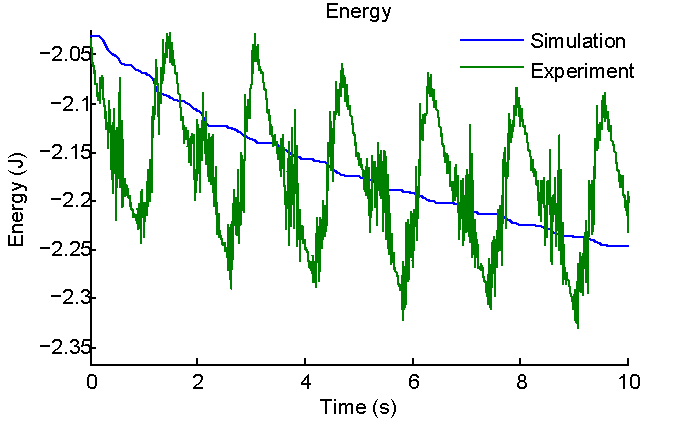
\includegraphics[scale=0.65]{comparison_energy_damped.pdf}
\caption{Comparison of energy over time for simulational and experimental data with damping.}
\label{energyresults}
\end{figure} 

The position and velocity as functions of time for each of the three pendulum links are shown in Figures \ref{positionresults} and \ref{velocityresults} for the tested periodic case.  As shown, the data matches up with the experimental results almost perfectly.

\begin{figure}[H]
\centering
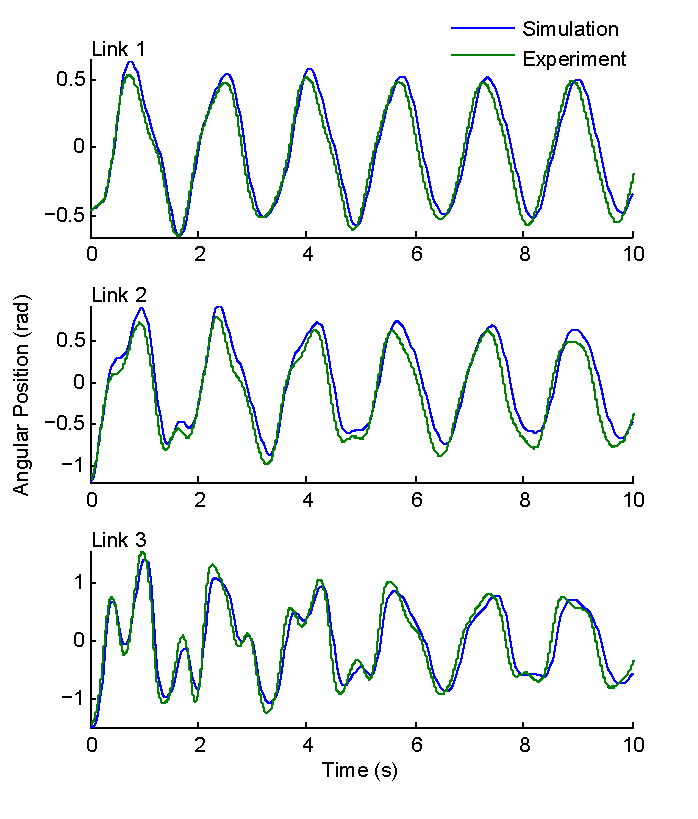
\includegraphics[scale=0.65]{comparison_position_damped.pdf}
\caption{Comparison of position over time for simulational and experimental data with damping.}
\label{positionresults}
\end{figure} 

\begin{figure}[H]
\centering
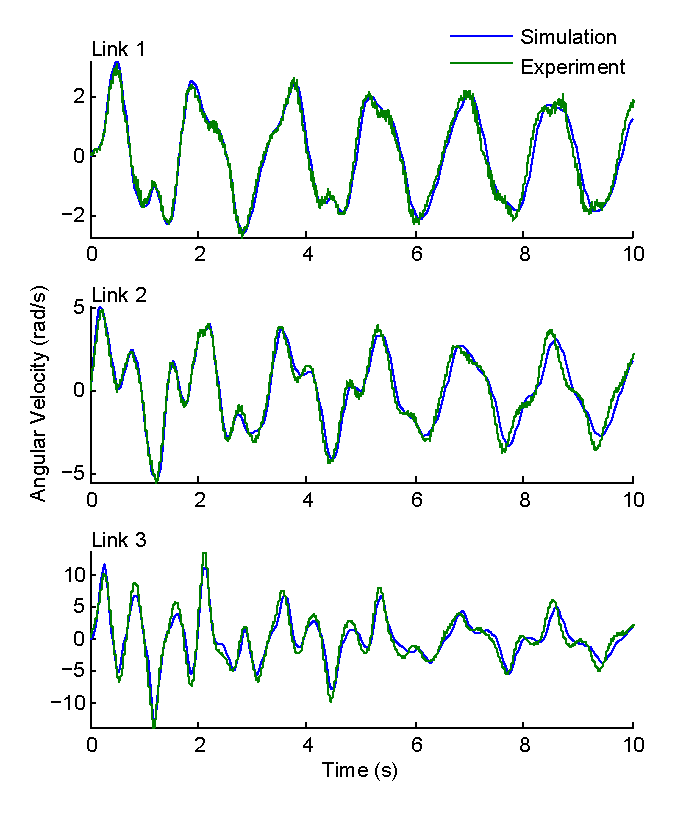
\includegraphics[scale=0.65]{comparison_velocity_damped.pdf}
\caption{Comparison of velocity over time for simulational and experimental data with damping.}
\label{velocityresults}
\end{figure}

When doing the double pendulum, we found that for chaotic systems the modeled and experimental results to separate quickly and postulated that this effect was due to damping in the system which our prior model did not take into account.  This hypothesis was tested by using our simulation to plot the paths of the triple pendulum masses for a set of chaotic initial conditions for both the damped and undamped case (Figure \ref{paths}).  Although there are definite qualitative similarities in the paths of the two masses, the addition of damping causes their paths to differ rather significantly and separate quickly after the first period of high kinetic energy.


\begin{figure}[H]
\centering
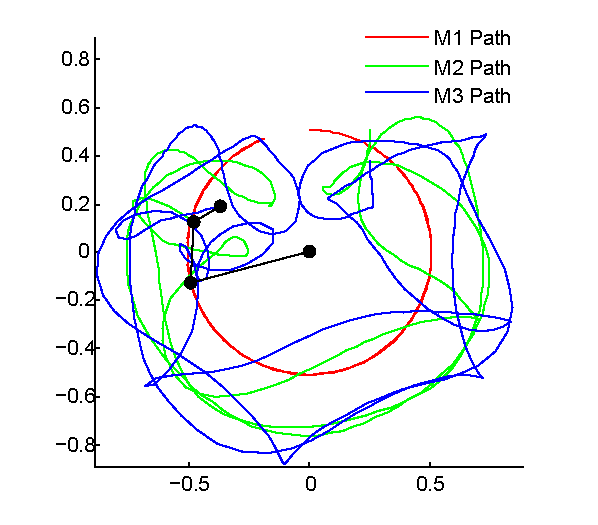
\includegraphics[scale=0.65]{path_nodamping.pdf}
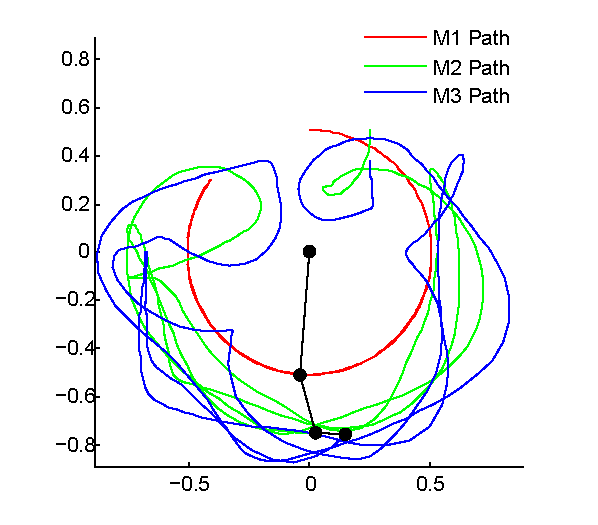
\includegraphics[scale=0.65]{path_damping.pdf}
\caption{The paths of the three links for both (a) undamped and (b) damped cases for a set of chaotic initial conditions.}
\label{paths}
\end{figure}


